
%{
%\setbeamertemplate{headline}{}
%\setbeamertemplate{footline}{}
%\usebackgroundtemplate{
%  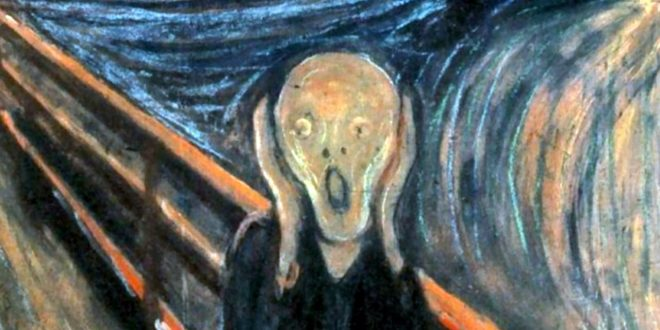
\includegraphics[width=\paperwidth]{munch2.jpg}
%}
%\begin{frame}
%\end{frame}
%}

%\section{Введение в Haskell}


%\defverbatim[colored]{\imageA}{
%\begin{tikzpicture}
%    [%%%%%%%%%%%%%%%%%%%%%%%%%%%%%%
%        box/.style={rectangle,draw=black, ultra thick, minimum size=1cm},
%    ]%%%%%%%%%%%%%%%%%%%%%%%%%%%%%%
%
%\foreach \x/\y in {0/9, 1/\faAmazon,2/13,3/19,4/12,5/8,6/7,7/4,8/21,9/2,10/6,11/11}
%        \node[box] at (\x,0){\y};
%
%\end{tikzpicture}
%}


\begin{frame}
  Алонзо Чёрч 1935   открыл $\lambda$-исчисление


  Аналогичный подход от А.Тьюринга с его машинами Тьюринга

  Всё формализация понятия алгоритма


  В принципе, могло быть изобретено уже в 1910х гг
\end{frame}

\begin{frame}{Состояние математики в 1910х}
  \begin{itemize}
    \item матан, алгебра, геометрия
    \item информатики существует неявно, как часть математики
    \item Математическая логика
    \begin{enumerate}
      \item Пытается формализовать интуитивно понятные утверждения
      \item Языки (т.е. синтаксис), чтобы на них можно было правильно сформулировать теоремы
      \item Различные интерпретации синтаксиса (т.е. семантики), потому что формулы могут быть верны и не верны в зависимости от семантики
      \item ``Исчисления'' -- правильные способы доказательств
      \item Теоремы, которые невозможно ни доказать, ни опровергнуть.
    \end{enumerate}
  \item Начинают задумываться, что такое ``алгоритм'', ``вычисление'' и ``вычислимая функция''.
  \end{itemize}
\end{frame}

\begin{frame}{Зачем формализовывать то, что и так понятно?}
  Например, любой школьник знает, что такое множество
  \begin{itemize}
    \item И множетсво множеств
    \item И множество множеств множеств
    \item ...
    \item И множество всех множеств
    \begin{enumerate}
\item       Но, необжиданно, множество всех множеств -- не множество!
      \item Парадок Рассела
      \item ДОказательство -- сведение к противоречию.
    \end{enumerate}
  \end{itemize}
\end{frame}

\begin{frame}{Пример: яызк 0го порядка (высказываний) }
\frametitle{Знакомая вам булева (бинарная) логика}

Тут описание языка

\begin{theorem}[Язык и исчисление хорошие]
  Верную формулу можно доказать за конечное число шагов.

   Ложную можно опровергнуть.

   Т.е. существует алгоритм, который говорит да/нет и всегда завершается
\end{theorem}

Язык и исчисление плохие, потому что не всё можно записать (где кванторы?)

\end{frame}


\begin{frame}{Язык и исчиследние 1го порядка (предикатов)}
\framesubtitle{Вы это видели на матане}

TODO: формальное описание

Пример: $\forall x z \exists y (x < y) \vee (y < z)$
верно, если $x,y,z \in \mathcal{R}$, неверно, если $x,y,z \in \mathcal{N}$

Мораль
\begin{itemize}
  \item Для некоторых формул из синтаксиса можно понять, что они верны (общезначимы). Для них есть алгоритм, который их докажет за конечное число шагов (метод британского музея)
  \item Огромное количество формул верны только в некоторой семантике, для них нельзя предъявить, алгоритм, который завершается и выдает вердикт
\end{itemize}
\begin{definition}[Разрешимая задача]
\end{definition}
\begin{definition}[Полуразрешимая задача]
\end{definition}
\end{frame}


\begin{frame}{Недостатки исчисления предикатов}
Некоторые формулы нельзя записать, а следовательно, пользоваться ими при доказательстве

Например, принцип индукции



Для этого нужен язык более высокого порядка, чем первого, а там всё ещё хуже с разрешимостью/неразрешимостью
\end{frame}

\section{Лямбды как апгрейд языка предикатов}

\begin{frame}{Но можно попробовать вывернуться}
\framesubtitle{Введем специальный синтаксис}

\[
\lambda P.\quad phormula(P)
\]
Опишем принцип индукции, и применим его для $P(n)\equiv 0+\dots+n=\frac{n\cdot(n+1)}{2}$
\[
\lambda P.\quad P(0) \Rightarrow (\forall n . P(n) \Rightarrow P(n+1))  \Rightarrow (\forall n . P(n))
\]
\[
\text{применение/подстановка} \mathlarger{\mathlarger{\mathlarger{\mathlarger{\Downarrow  \quad\Uparrow}}}} \text{абстракция}
\]

\begin{equation} \label{eq1}
  \begin{split}
    (0\equiv0) & \Rightarrow (\forall n . (0+\dots+n=\frac{n\cdot(n+1)}{2}) \Rightarrow \Big{(}0+\dots+(n+1)=\frac{(n+1)\cdot(n+2)}{2}\Big{)})  \\
    & \Rightarrow (\forall n . 0+\dots+n=\frac{n\cdot(n+1)}{2})
  \end{split}
\end{equation}
\end{frame}



\begin{frame}{Правила работы с новым языком $\lambda$}
\begin{block}{$\alpha$-эквивалентность}
При выборе новых имен, они не должны случайно перекрыть старые.\\
Предложения языка, отличающиеся только переименованием переменных, считаются ($\alpha$)эквивалентными
\end{block}
Например:  если ни $P$, ни $Q$ не встречаются в $phormula$, то $\lambda P. phormula(P)  \alphaequiv{} \lambda Q. phormula(Q) $

\begin{block}{$\beta$-эквивалентность}
Если у нас встречается $(\lambda P. phaormula(P))X$, то мы можем продолжить с этим работать, используя $phormula[P\mapsto X]$, т.е. заменив все свободных вхождения $P$ на $X$ внутри $phormula$
\end{block}
\end{frame}


\begin{frame}{$\lambda$-исчсисление}
 TODO: определение


 Так получилось, что если добавить в язык синтаксис абстракции, применения, и имена перменных, по-видимому, на этом можно записать произвольный алгоритм

 \begin{theorem}[Тезис Чёрча]
   Используя $\lambda$ исчисление можно реализовать произвольный алгоритм, с точностью до представления данных.
 \end{theorem}
\end{frame}


\section{Две стратегии}

\begin{frame}{Как происходят вычисления $\lambda$-исчислении?}
\begin{definition}[Процесс вычислений регламентирует стратегия]
  Ищем редексы $(\lambda x. P)Q$
\begin{itemize}
  \item Если редексов нет, то вычисление закончилось
  \item Если редексы есть, стратегия регламентирует какой на данном шаге редекс стоит $\beta$редуцировать
  \item Или же, стратегия может сказать, что все редексы нужно оставить как есть, и выдать ответ.
\end{itemize}
\end{definition}
Стратегий бывает много разных
\begin{enumerate}
  \item Строгая стратегия call-by-value .    Для $(\lambda x. P)Q$ вычисляет $Q\cbv Q'$ и потом подставляет $Q'$ вместо $x$ в $P$.
  \item Ленивая стратегия call-by-name.   Для $(\lambda x. P)Q$ сразу подставляет $Q$ вместо $x$ в $P$.
  \item Обе стратегии оставляют абстракции и переменные как есть
\end{enumerate}


\end{frame}

\begin{frame}{Ленивая vs. Строгая}
Пример 1 ($\cbv$ выглядит лучше)\\
$(\lambda x. f x x)((\lambda x. x)A) \cbv (\lambda x. f x x)A \cbv (f A A) \cbv \dots $\\

$(\lambda x. f x x)((\lambda x. x)A) \cbn (\lambda x. f ((\lambda x. x)A) ((\lambda x. x)A))A \cbn \dots $

\vspace{3em}
Пример 2 ($\cbn$ выглядит лучше)\\
$(\lambda x. \lambda y. y)((\lambda x. xx)(\lambda x. xx)) \cbv (\lambda x. \lambda y. y)((\lambda x. xx)(\lambda x. xx)) \cbv \dots \text{зависло}$

$(\lambda x. \lambda y. y)((\lambda x. xx)(\lambda x. xx)) \cbn (\lambda y. y)\quad\text{ответ!}$
\end{frame}

\section{Представление данных в $\lambda$ исчислении}
\begin{frame}{Представление данных}
  Нумералы Чёрча
$ 0 \sim \lam{s}{\lam{x}{x}}$

$ 1 \sim \lam{s}{\lam{x}{sx}}$

$ 2 \sim \lam{s}{\lam{x}{s(sx)}}$

и т.д.
\vspace{1cm}

Сложение (один из вариантов): взять два нумерала $m$ и $n$, взяьб $f$ и $x$, а затем к $x$ применить $n$ раз $f$, а затем к результату применить $m$ раз $f$.

\[
add \equiv \lambda m. \lambda n. \lambda f. \lambda x. \app{m\ f\ }{\app{n\ f\ }{x}}
\]
\end{frame}
\newcommand{\tb}[1]{\textcolor{blue}{#1}}
\newcommand{\tr}[1]{\textcolor{red}{#1}}
\begin{frame}{2+2}
  \begin{align*}
    (\lambda m. \lambda n. \lambda f. \lambda x. \app{m\ f\ }{\app{n\ f\ }{x}}){} 2 2 &\cbv \\
    \textcolor{blue}{(\lambda m. \lambda n. \lambda f. \lambda x. \app{m\ f\ }{\app{n\ f\ }{x}}) {}} \textcolor{red}{2} 2 &\cbv \\
    \textcolor{blue}{( \lambda n. \lambda f. \lambda x. \app{2\ f\ }{\app{n\ f\ }{x}}){}} \textcolor{red}{2} & \cbv \\
    \lambda f. \lambda x. \app{2\ f\ }{\app{2\ f\ }{x}}   &\xarr{\ \ } \\
    \lambda f. \lambda x. \app{\tb{\lam{f}{\lam{x}{f (f x)}}} \ \tr{f}\ }{\app{2\ f\ }{x}} &\ao \\
    \lambda f. \lambda x. \app{\lam{x}{f (f x)} \ \ }{\app{2\ f\ }{x}} &\xarr{\ \ } \\
    \lambda f. \lambda x. \app{\lam{x}{f (f x)} \ \ } {\app{\app{\tb{\lam{f}{\lam{x}{f (f x)}}}\ \tr{f}\ }{x}}} &\ao \\
    \lambda f. \lambda x. \app{\lam{x}{f (f x)}  } {\app{\tb{\lam{x}{f (f x)} } }{\tr{x}}} &\ao \\
    \lambda f. \lambda x. \app{\tb{\lam{x}{f (f x)} } } {\tr{(f (f x))}} &\ao \\
    \lambda f. \lambda x. \lam{x}{f (f (f (f x)))} &
  \end{align*}
\end{frame}


\begin{frame}{2+2}
  \begin{figure}[t]
    \begin{subfigure}[t]{0.50\textwidth}
  \begin{align*}
  (\lambda m. \lambda n. \lambda f. \lambda x. \app{m\ f\ }{\app{n\ f\ }{x}}){} 2 2 &\cbv \\
  \textcolor{blue}{(\lambda m. \lambda n. \lambda f. \lambda x. \app{m\ f\ }{\app{n\ f\ }{x}}) {}} \textcolor{red}{2} 2 &\cbv \\
  \textcolor{blue}{( \lambda n. \lambda f. \lambda x. \app{2\ f\ }{\app{n\ f\ }{x}}){}} \textcolor{red}{2} & \cbv \\
  \lambda f. \lambda x. \app{2\ f\ }{\app{2\ f\ }{x}}   &
\end{align*}
Это ответ для $\cbv$.\\

Давайте посмотрим, что будет, если мы \\
ответ применим к $g$ и $y$
    \end{subfigure}
    \begin{subfigure}[t]{0.45\textwidth}
  \begin{align*}
  (\lambda f. \lambda x. \app{2\ f\ }{\app{2\ f\ }{x}}) g y  &\cbv \\
  (\lambda x. \app{2\ g\ }{\app{2\ g\ }{x}}) y  &\cbv \\
  \app{2\ g\ }{\app{2\ g\ }{y}}   &\cbv \\
  \app{\tb{\lam{f}{\lam{x}{f (f x)}}} \ \tr{g}\ }{\app{2\ g\ }{y}} &\cbv \\
  \app{\lam{x}{g (g x)} \ \ }{\app{2\ g\ }{y}} &\cbv \\
  \app{\lam{x}{g (g x)} \ \ } {\app{\app{\tb{\lam{f}{\lam{x}{f (f x)}}}\ \tr{g}\ }{x}}} &\cbv \\
  \app{\lam{x}{g (g x)}  } {\app{\tb{\lam{x}{g (g x)} } }{\tr{y}}} &\cbv \\
  \app{\tb{\lam{x}{g (g x)} } } {\tr{(g (g y))}} &\cbv \\
  g (g (g (g y))) &
\end{align*}
    \end{subfigure}
  \end{figure}

\end{frame}

\begin{frame}{Ветвления}
\[
T\equiv\lam{x}{\lam{y}{x}} \equiv fst \qquad \qquad \qquad \qquad
F\equiv \lam{x}{\lam{y}{y}}\equiv snd
\]

  \begin{align*}
  ite \equiv & \lambda c. \lambda th. \lambda el. (c\ th\ el) \\
  (ite\ T) \equiv &  \lambda th. \lambda el. (T\ th\ el) \cbn th\\
  (ite\ F) \equiv &  \lambda th. \lambda el. (F\ th\ el) \cbn el
\end{align*}


\end{frame}

\newcommand{\ite}[3]{\ensuremath{(\text{if } #1\text{ then }#2\text{ else }#3})}}
\begin{frame}{Рекурсия в call-by-name}
$$
Y\equiv \lam{f}{\lam{x}{f(xx)}\lam{x}{f(xx)}}
$$
%Основное свойство
\[
YR = \lam{x}{R(xx)} \lam{x}{R(xx)} \nor
R\big( \lam{x}{R(xx)}\lam{x}{R(xx)} \big) =
R(YR)
\]

\vspace{1em}

Факториал: $fac \equiv (\lambda self.\lambda n . \ite{n<2}{1}{n \cdot self(n-1)})$
\begin{align*}
  Y(\lambda self.\lambda n . \ite{n<2}{1}{n \cdot self(n-1)}) 2 &\cbn \\
  (\lambda n . \ite{n<2}{1}{n \cdot Y\ fac(n-1)}) 2 &\cbn \\
   2 \cdot Y\ fac\ (2-1) &\cbn \\
   2 \cdot (Y(\lambda self.\lambda n . \ite{n<2}{1}{n \cdot self(n-1)})\ 1) &\cbn \\
   2 \cdot \ite{1<2}{1}{n \cdot (Y\ fac\ (1-1))} &\cbn \\
  2 \cdot 1 & \cbn 2
\end{align*}

\end{frame}

\section{Демка интерпретатора на Си}
\begin{frame}{Дэмка на Си}
  Не забыть показать позднее связывание
\end{frame}

\section{Вопросы к экзамену}
\begin{frame}{Вопросы к экзамену}
\begin{enumerate}
  \item Разрешимые и неразрешимые задачи
  \item $\lambda$-исчисление. $\alpha$ и $\beta$ правила
  \item Нумералы Чёрча. Сложение
  \item Рекурсия и факториал
\end{enumerate}
\end{frame}

%
%\begin{frame}%{Чистые функции}
%\begin{definition}[Неизменяемые структуры данных (immutable data structures)]
%  Которые с течением времени не изменяются \faSmileO
%\end{definition}
%
%\vspace{1em}
%
%\begin{definition}[Устойчивые структуры данных (persistent data structures)]
%Имеют доступ (не уничтожают) предыдущее своё состояние
%\end{definition}
%Почти то же самое, только акцент смещён\vspace{1em}
%
%\begin{remark}
%Так как старые узлы есть, то можно их использовать (share) в новой версии структуры данных
%\end{remark}
%\begin{definition}[Неустойчивые структуры данных называются \textit{эфемерными (ephemeral)}]
%\end{definition}
%\end{frame}

